\chapter{二维材料异质结生长机理的研究}
\section{引言}
\section{计算细节}
\section{石墨烯/六方氮化硼纵向二维异质结的生长机理}

    \begin{figure}[htb]
        \subfloat[]{
            \centering
            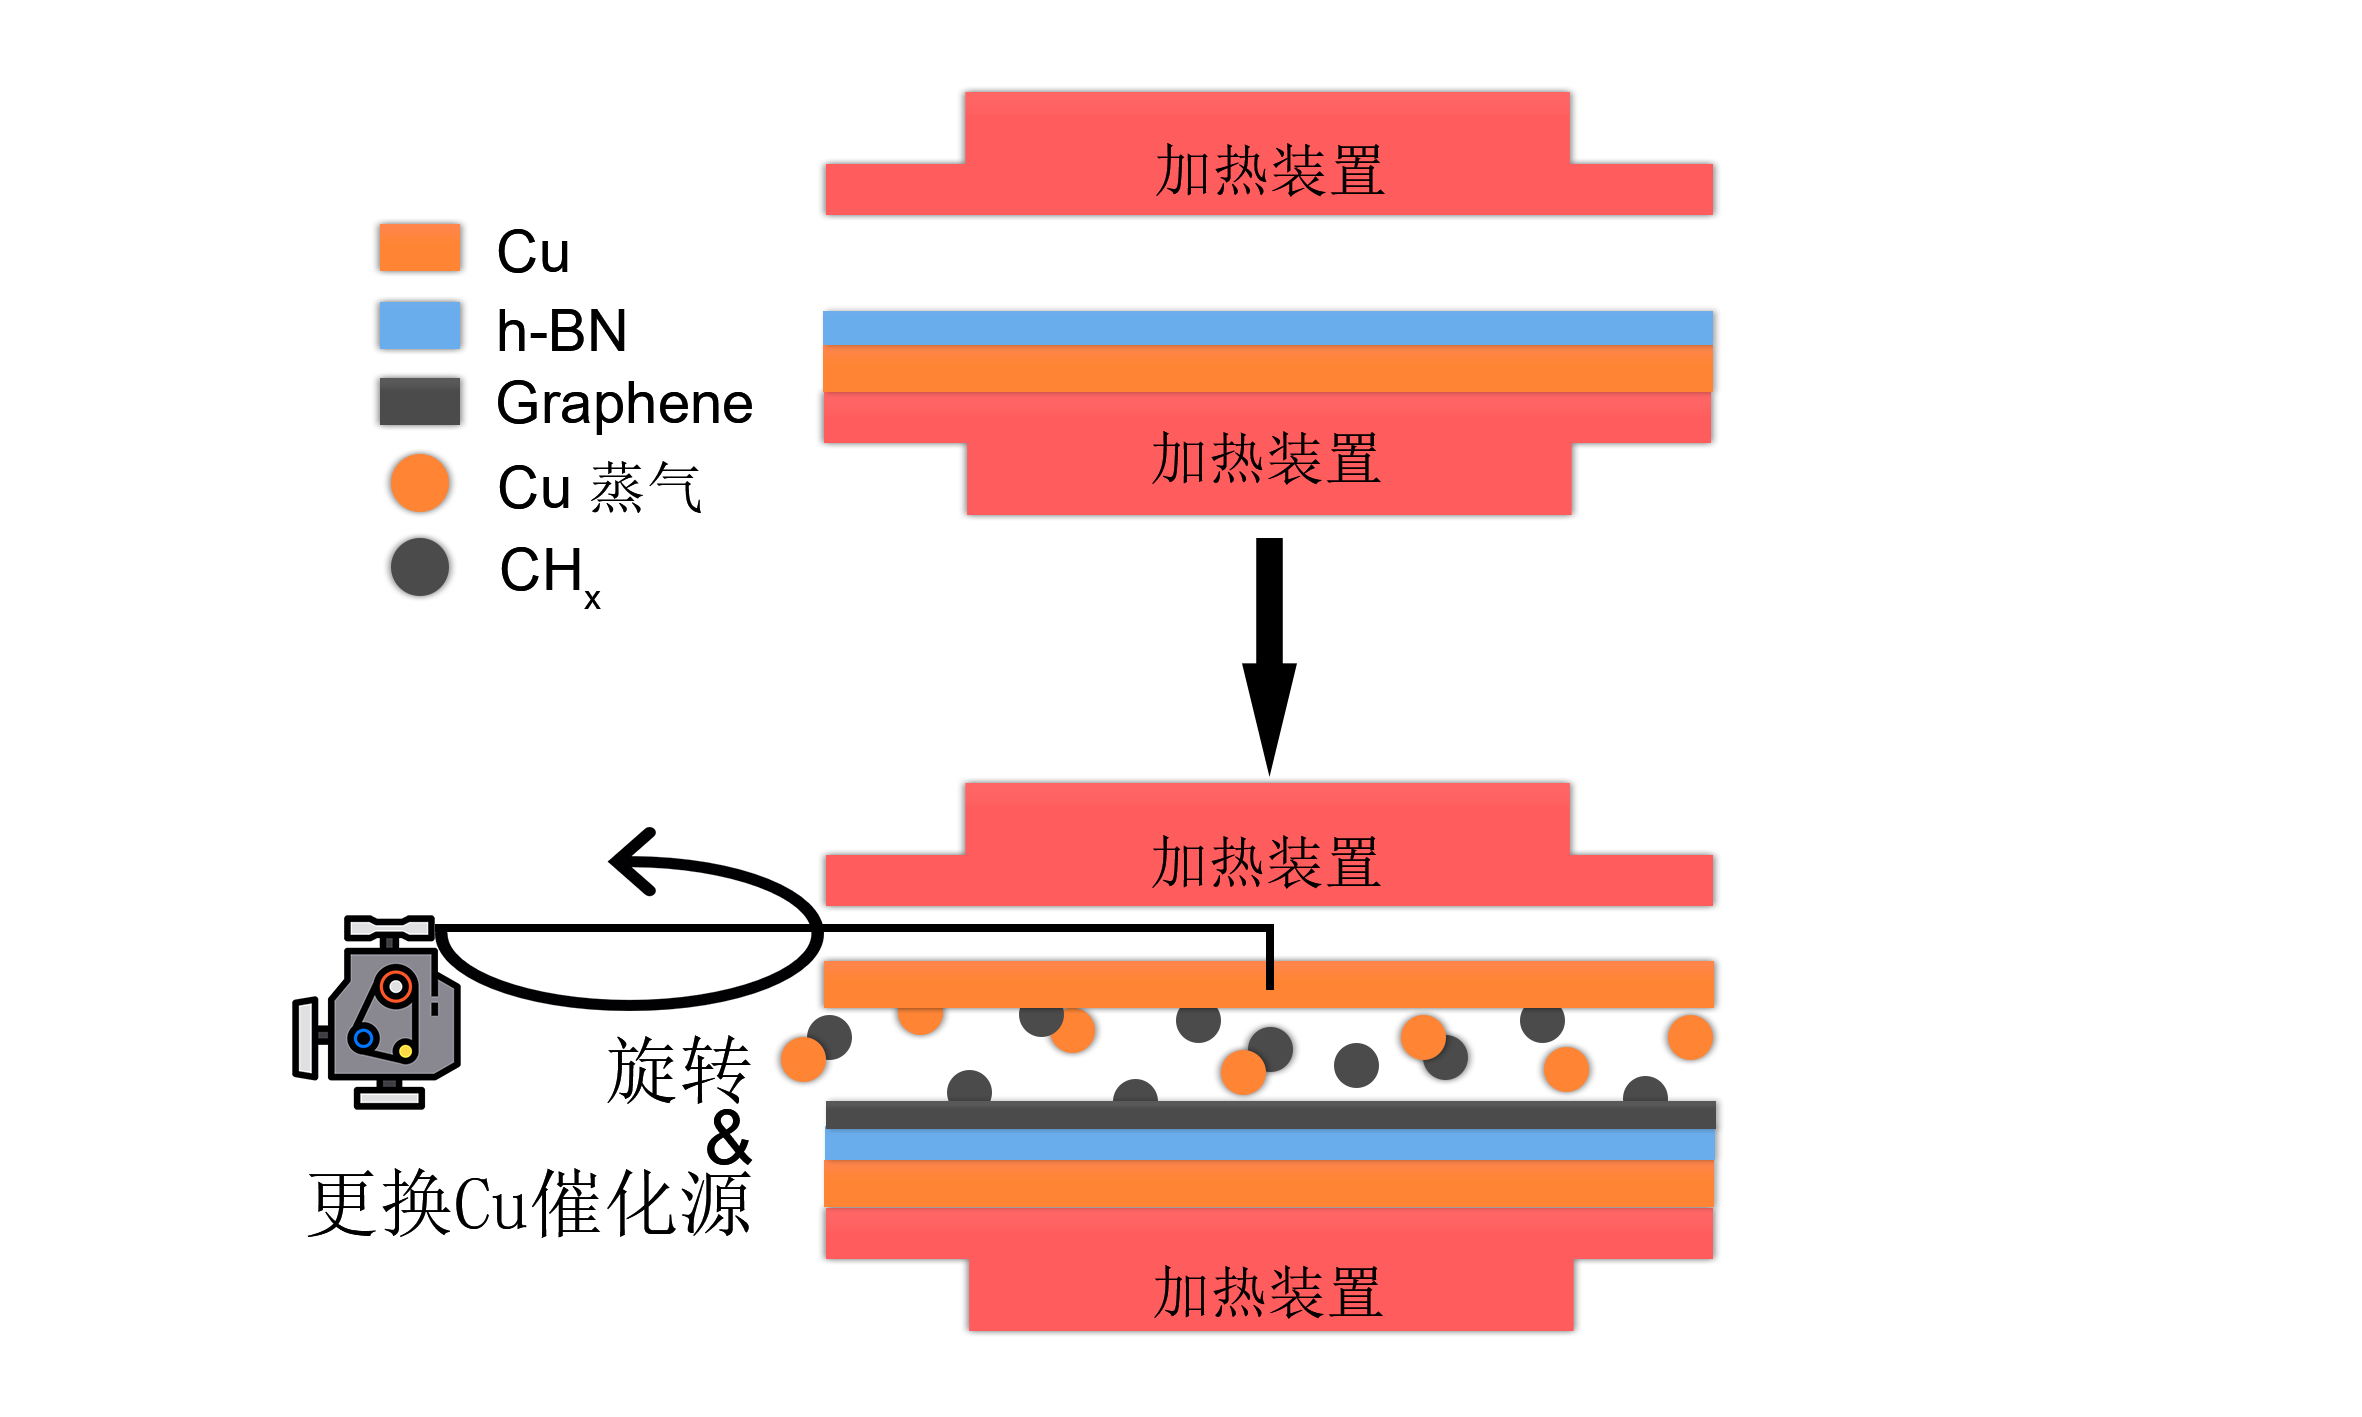
\includegraphics{pic/CG_diagram_routine.png}
            \label{fig:CG_diagram_routine}
        }
        \newline
        \subfloat[]{
            \includegraphics{pic/CG_diagram_growthSketch.png}
            \label{fig:CG_diagram_growthSketch}
        }
        \caption{利用铜蒸气近邻催化效应在六方氮化硼表面直接堆叠生长石墨烯。(a)生长装置示意图;(b)石墨烯/六方氮化硼异质结生长过程示意图}
        \label{fig:CG_diagram_CVD}
    \end{figure}

    \subsection{近邻蒸发气态铜催化剂的扩散}
    
    \begin{figure}[htb]
        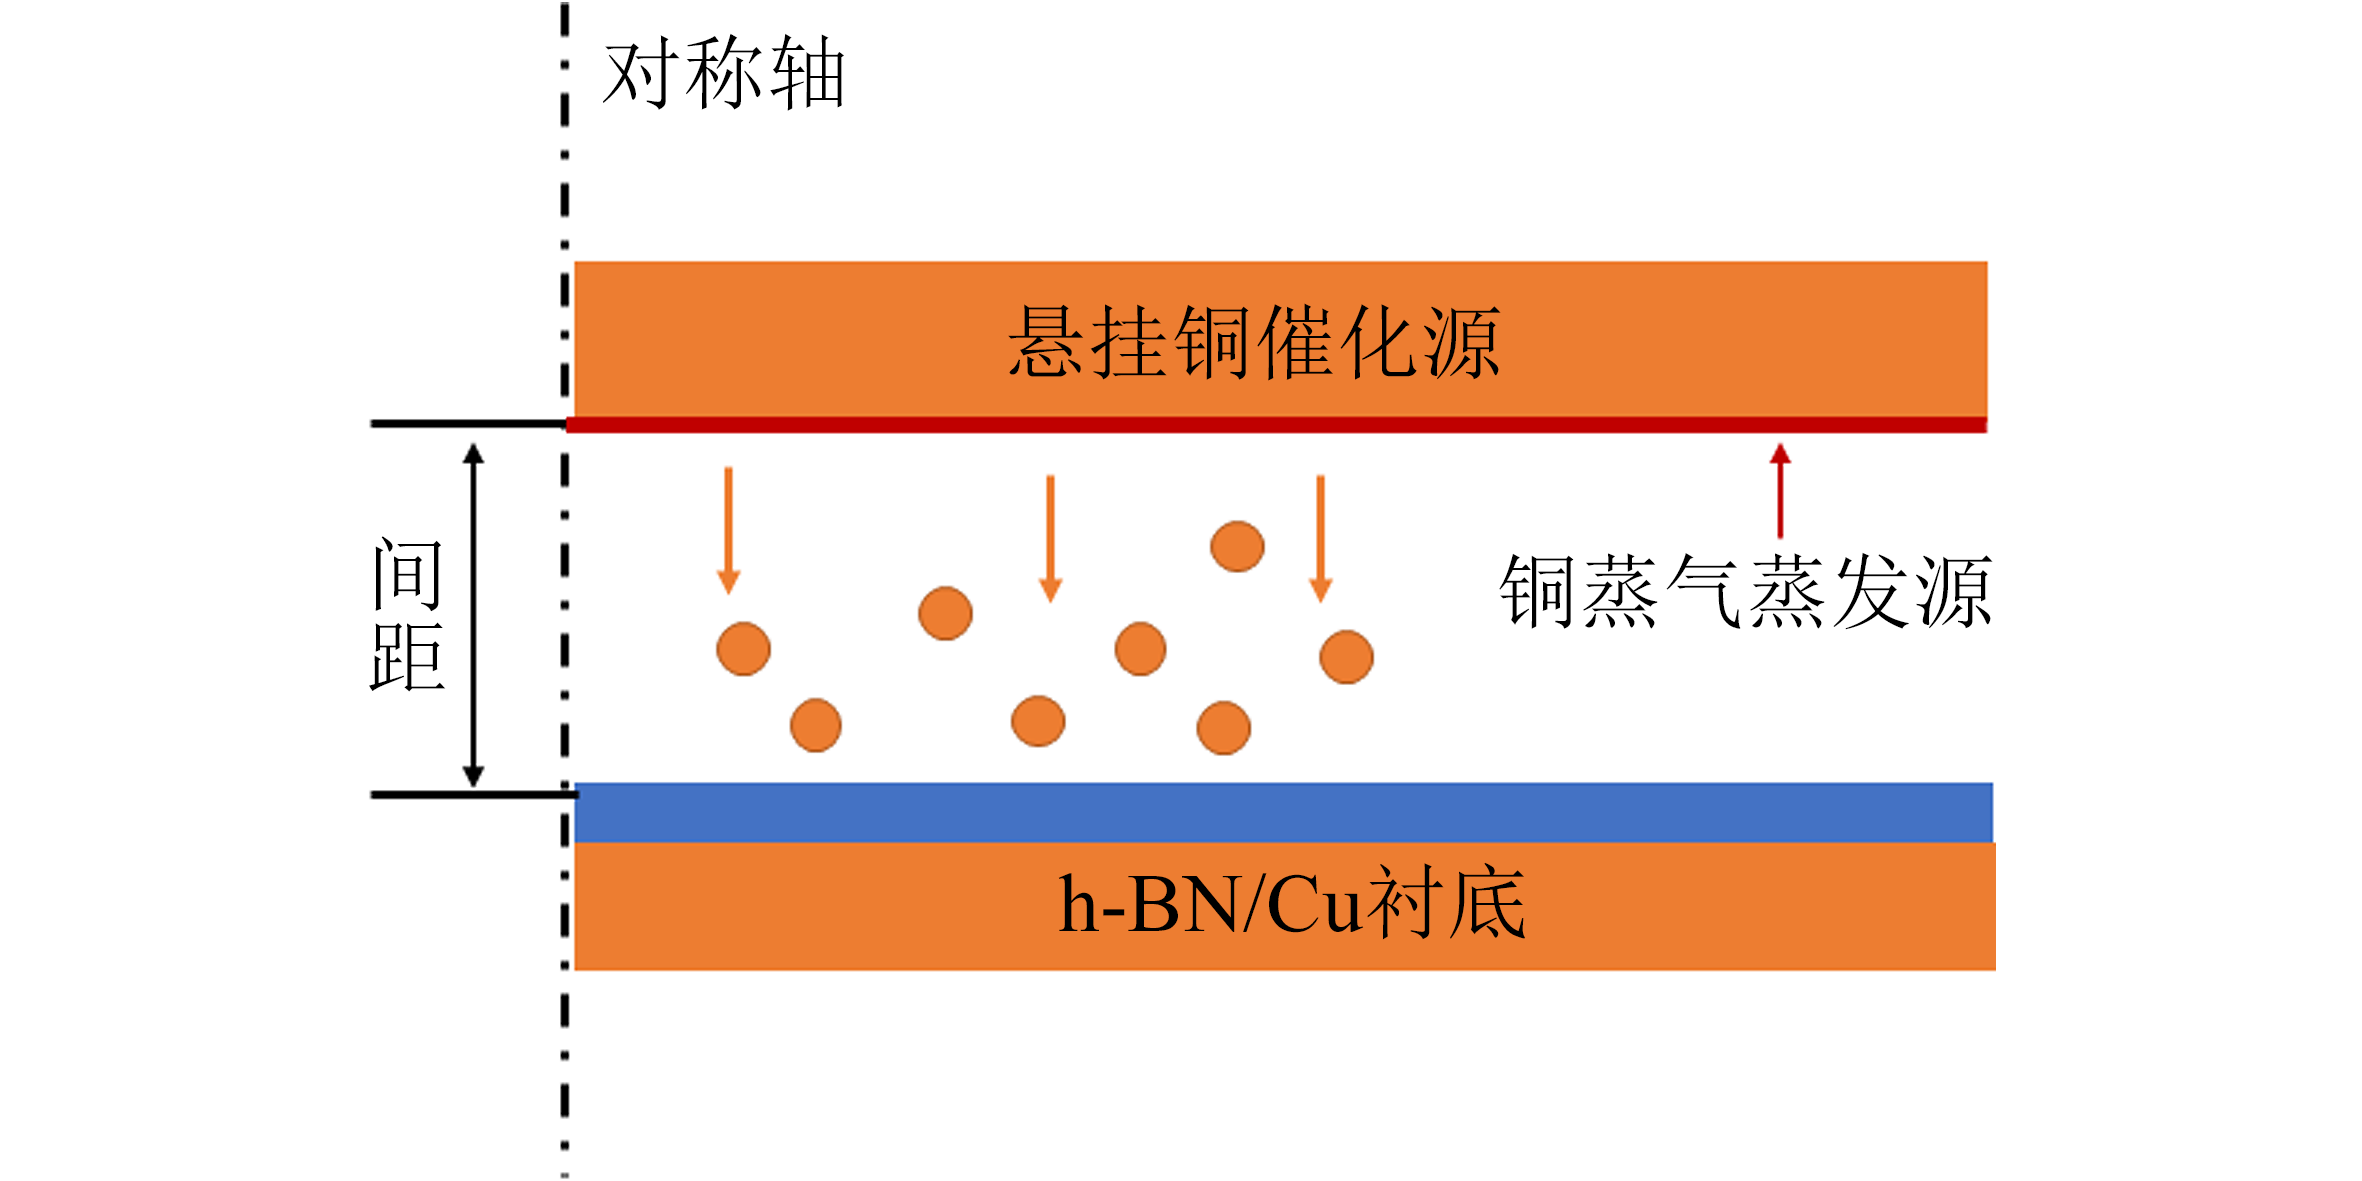
\includegraphics{pic/CG_diagram_FEM_structure.png}
        \caption{化学气相沉积腔体内铜蒸气扩散模拟示意图。}
        \label{fig:CG_diagram_FEM_structure}
    \end{figure}

    \begin{figure}[htb]
        
    \end{figure}

    \subsection{气态铜催化剂对甲烷裂解反应的催化性能}
    \subsection{六方氮化硼表面石墨烯的生长演化机理}
\section{石墨烯/二硒化钒横向异质结的生长机理}
\section{总结}